\chapter{Neutrino Unfolding}
\label{ch:gnns}

Particle physics experiments have finite resolution, limited acceptance, and error-prone reconstruction algorithms.
These limitations mean that the actual physical variable of interest $\x$ and its associated distribution $p_\text{gen}(\x)$ are not directly observable.
Instead, we only have access to some distorted reconstructed proxy $\y$ and its distribution $p_\text{data}(\y)$.
MC Simulations can use theoretical assumptions to make predictions on the expected distribution $p_\text{MC} \approx p_\text{gen}$, and then expensive detector simulations are run to estimate,
\begin{equation}
    \int p_\text{detector}(\y|\x) p_\text{MC}(\x) \diff\x \approx p_\text{data}(\y).
\end{equation}
The inverse of this process, relating $p_\text{data}(\y)$ to $p_\text{gen}(\x)$, is called unfolding.
Unfolding is useful as it allows a comparison between predicted theory and observed data in a way that is independent of the detector response.
If one has access to the reverse process $p_\text{unfold}(\x|\y)$, then one can use it to unfold the data by,
\begin{equation}
    p_\text{gen}(\x) = \int p_\text{unfold}(\x|\y) p_\text{data}(\y) \diff\y.
\end{equation}
This however is a difficult, and ill-possed task: the solutions are not unique, and small changes in $p_\text{data}$ can cause large changes in the $p_\text{gen}$.

In this chapter we describe the work done to create deep generative models to approximate $f_\theta(\y) \approx p_\text{unfold}(\x|\y)$.
Specifically, we focus on the problem of unfolding the momentum of the neutrinos in the final state of the event.
This is a specifically challenging setting as neutrinos are not directly observable in data.
Their experimental signature $\ptmiss$, described in \Cref{sec:MET}, only captures a noisy approximation of the net neutrino momentum in the transverse plane.

This chapter summarizes the work done in \textcite{NuFlows1} and \textcite{Nu2Flows}, which describes the development for models to unfold the neutrino momentum in events with one and two neutrinos in the final state, respectively.

\section{Introduction}

Neutrinos couple solely to the weak nuclear force and do not interact with detector material; they escape collider experiments undetected.
Their presence is inferred from the missing transverse momentum $\ptmiss$, calculated from the momentum imbalance of all visible particles in the plane perpendicular to the beam pipe.
This variable is an experimental proxy for the net transverse momentum of all undetected particles.
However, no such proxy exists in the longitudinal direction due to the unknown initial momentum of the colliding partons.
Even with accurate $\ptmiss$ reconstruction, events producing multiple neutrinos leave their all individual kinematics under-constrained.

Analyses in collider physics often involve neutrino production and would benefit from determining the individual kinematics of final-state neutrinos.
A notable example is the study of the top quark, which decays almost instantaneously into a $b$-quark and a $W$ boson in 99.9\% of cases.
Approximately one-third of these $W$ bosons decay leptonically, resulting in a final state that includes a neutrino.
As the heaviest particle in the Standard Model, the top quark has the largest coupling to the Higgs boson.
It plays a unique role in the stability of the electroweak vacuum due to its presence in the quadratic term of the Higgs potential.
Its rapid decay offers a unique opportunity to measure the properties of a bare quark.

Reconstructing the $\ttbar$ system, including top quarks decaying leptonically via a $W$ boson, is crucial for many top quark measurements.
However, the unknown momentum of final-state neutrinos makes it impossible to reconstruct the event entirely.

Our method utilizes a deep generative model to approximate the set of neutrino momenta $\{\p^{\nu_i}\}_{i=1}^N$, given all observable objects in the event and the number of neutrinos $N$.
It is trained on simulated events with known neutrino momenta.
Standard deep learning regression methods collapse the posterior into a point estimate, failing to capture solution diversity or uncertainty.
Therefore, a probabilistic approach that provides the likelihood over a range of viable solutions is necessary.

We use a normalizing flow (NF), detailed in \Cref{sec:flows}.
For this task, the NF requires observed data and two main underlying assumptions or implicit biases: the physical process being studied, ingrained into the flow by the training set's composition, and the assumed number of neutrinos or non-interacting particles, built into the flow's structure.
These assumptions are crucial to constraining the solution space.

We call our method~\nuflow, and it is composed of two key networks.
The first is an invertible neural network which learns a bijection between truth neutrino momenta and the latent space, each represented as flattened rank-1 tensors, given a context tensor.
The second is a feature extractor, which learns an expressive context tensor given all the visible objects in the event.
Much of the work throughout these projects involved expanding and testing more sophisticated feature extractors.

\section{Single Neutrino Final State}

The simplest case is when there is only one neutrino in the final state which has three dimensions and we use the semi-leptonic $\ttbar$ decay as a case study\footnote{The code~\cite{SemileptonicTtbarNeutrino} and datasets~\cite{NuFlowsCode} are publicly available.}.
The final-state of this process contains at least four jets, a lepton, and a single neutrino as shown in \Cref{fig:feynman}.

\begin{figure}[ht]
    \center
    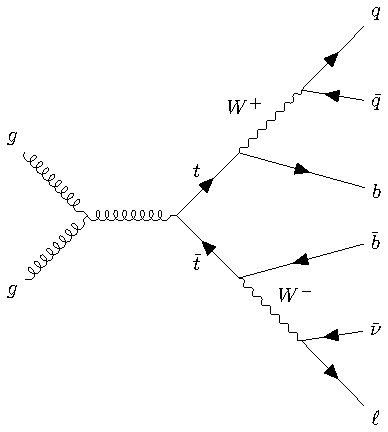
\includegraphics[width=0.4\textwidth]{Figures/neutrino_unfolding/feynman.pdf}
    \caption{A representative Feynman diagram illustrating the semi-leptonic decay of a top quark pair produced the gluon-gluon fusion.}
    \label{fig:feynman}
\end{figure}

\subsection{Quadratic Solution}

For this process, the standard approach~\cite{Quad1, Quad2, Quad4, Quad5} to estimate $\p^\nu$ uses a kinematic constraint,
\begin{equation}
    \label{eq:quadratic}
    p_z^\nu = \frac{-b \pm \sqrt{b^2-4ac}}{2a}, \quad \text{where} \quad
    \begin{aligned}
        \alpha &= m_W^2 - m_\ell^2+2(p_x^\ell p_x^\nu+p_y^\ell p_y^\nu) \\
        a &= (p_z^\ell)^2 - (E^\ell)^2, \\
        b &= \alpha p_z^\ell, \\
        c &= \frac{\alpha^2}{4}-(E^\ell)^2(\pt^\nu)^2.
    \end{aligned}
\end{equation}
Here $(p_x^\ell, p_y^\ell, p_z^\ell, E^\ell)$ is the lepton's four-momenta with mass $m_\ell$, and $\pt^\nu$ is the transverse momentum of the neutrino, estimated by $|\ptmiss|$.

This approach has several drawbacks.
It assumes an exact $m_W$, introducing bias by ignoring its natural width.
It also assumes $\pt^\nu$ is perfectly captured by $\ptmiss$, overlooking misidentification and resolution effects.
These factors can result in complex solutions where the convention is to drop the imaginary component.
Additionally, even with perfect reconstruction, the equation will yield two real solutions, with no reason to favour one over the other, though the smaller magnitude result is typically taken.

\subsection{Data}

The data in this study comprises simulated $\ttbar$ events where exactly one top quark decays into a $b$-jet and a leptonically decaying $W^\pm$ boson, resulting in final states with $(e,\nu_e)$, $(\mu,\nu_\mu)$, or their antiparticles.
Around 600k events are used to train the model and an additional 100k events are used for evaluating performance.

\subsection{Monte Carlo Generation}

All events are generated from proton-proton collisions at a center-of-mass energy of $\sqrt{s} = 13~\TeV$.
Hard interactions are simulated using MadGraph5 3.1.0~\cite{MadGraph}, with decays of top quarks and $W$~bosons modelled with MadSpin~\cite{MadSpin}.
The mass of the top quark is set to $m_t = 173~\GeV$.
Event generation is interfaced to \textsc{Pythia 8.243}~\cite{Pythia8} to model parton shower and hadronisation.
All steps use the \textsc{NNPDF2.3LO} PDF set~\cite{PDF2.3} with $\alpha_S(m_Z) = 0.130$, as provided by the LHAPDF~\cite{LHAPDF6PartonDensity} framework.
The detector response is simulated using \textsc{Delphes 3.4.2}~\cite{Delphes} with a parametrization that mimics the response of the ATLAS detector.
Jets are reconstructed using energy-flow objects and the anti-$k_t$ algorithm~\cite{AntiKt} with a radius parameter of $R = 0.4$ using FastJet~\cite{FastJet}.
Jet $b$-tagging at $\bnom$ is used to identify jets originating from $b$-quarks.

\subsection{Event Selection}

Events are required to contain exactly one reconstructed electron or muon with $p_\mathrm{T} > 15~\GeV$ in the range $|\eta|<2.5$ and at least four jets with $\pt > 25~\GeV$ in the range $|\eta|<2.5$.
At least two of the jets are required to pass the $b$-tagging criteria.
For truth labelling, jets were matched to partons within a radius of $\Delta R < 0.4$.
Events containing jets matched to multiple partons were removed from the training and evaluation datasets.

\subsection{Input and Target Features}

Variables from event reconstruction are used as conditioning inputs to the feature extractor network.
Up to 10 jets, as ordered by $p_\mathrm{T}$, are selected per event.
The full set of observed features is described in Table~\ref{tab:inputs}.
The target for the flow is the neutrino three-momentum vector defined by $(p_x^\nu, p_y^\nu, \eta^\nu )$.
The coordinate system used to represent the momentum of each physics object, was optimized as part of a hyperparameter scan.
We found that using $\eta$ instead of $p_z$ and the logarithm of the energy $\log E^j$ yielded the best performance.
We use standard normalization techniques to scale the inputs and targets to zero mean and unit variance.

\begin{table}[ht]
    \caption{The observable inputs used for the event feature extractor.}
    \label{tab:inputs}
    \centering
    \begin{tabular}{r c l}
    \toprule
    Category & Variables & Description\\
    \midrule
    $\ptmiss$ & $p_x^\text{miss}$, $p_y^\text{miss}$ & Missing transverse momentum 2-vector \\ [2ex]
    \multirow{2}{*}{Lepton} & $p_x^{\ell}$, $p_y^{\ell}$, $\eta^\ell$, $\log E^\ell$ & Lepton momentum 4-vector \\
    & $\ell^{flav}$ &  Whether lepton is an electron or muon \\ [2ex]
    \multirow{2}{*}{Jets} & $p_x^{j}$, $p_y^j$, $\eta^j$,  $\log E^j$ & Jet momentum 4-vector \\
    & $isB$ &  Whether jet passes $b$-tagging criteria \\ [2ex]
    Misc & $N_{\text{jets}}$, $N_{\text{bjets}}$ & Jet and $b$-jet multiplicities in the event\\
    \bottomrule
    \end{tabular}
\end{table}

\subsection{Model Architecture}

The $\nuflow$ architecture optimized for this process is depicted in \Cref{fig:flow}.
All observed inputs are passed through a feature extractor network to produce a context tensor for the flow.
As there are a variable number of jets in each event, they are first passed through a multi-headed conditional deep set network.
The NF was constructed from of seven rational-quadratic spline coupling layers~\cite{NeuralSplineFlows} interleaved with LU-parameterized linear layers.
The latent distribution was chosen to be $\mathcal{N}(0, I)$.

\begin{figure}[ht]
    \centering
    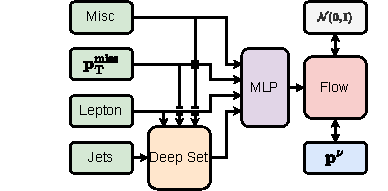
\includegraphics[width=0.49\textwidth]{Figures/neutrino_unfolding/nuflow.pdf}
    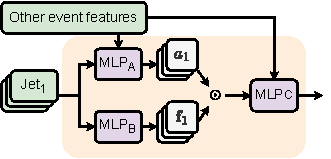
\includegraphics[width=0.3\textwidth]{Figures/neutrino_unfolding/deepset.pdf}
    \caption{The architecture of the $\nuflow$ model for the single neutrino case (left), and the attention weighted deep set used in the feature extractor (right).}
    \label{fig:flow}
\end{figure}

The model was constructed using the nflows library~\cite{nflows} and trained using the standard negative log-likelihood loss function.
A cosine annealing scheduler adjusted the learning rate from zero to $5\times 10^{-4}$ every two epochs.
Gradient clipping with a max-norm of 5 ensured stable convergence.
For cross-validation, $10\%$ of the training data was reserved as a holdout set, and early stopping was applied using a 30-epoch patience parameter.
We used the Adam optimizer~\cite{Adam} with default parameters and a 256 batch size.
The training was done on an NVIDIA 2080-Ti GPU, with the NF taking around 4 hours to converge.

To compare performance with standard regression, we also trained a feed-forward network (FF) using only the feature extractor to predict the neutrino three-momentum directly.
The FF network was trained using Smooth-L1 loss function~\cite{SmoothL1}.
All other training parameters were kept the same.
This approach is termed \nuff{}\@.

\subsection{Results}
\newcommand{\nusample}{\nuflow(\text{sample})}
\newcommand{\numode}{\nuflow(\text{mode})}

For unfolding, we sample under the flow in reverse-mode, and we call this method \nusample.
This method has low bias but high variance.
Alternatively, we can approximate $\arg\max_\X{p_X(\x|\con)}$ by generating 256 neutrinos per event and selecting the solution with the highest likelihood.
We call this method \numode.
We compare these methods to the mass constraint solution and \nuff.
Furthermore, we include reconstruction using the true neutrino momenta; plots labelled \emph{Truth} refer only to the neutrino values, while other properties, such as those of leptons or jets, are from reconstructed objects.

\Cref{fig:inference} illustrates the benefits of \nuflow{} by comparing the reconstruction methods in $\nu^\eta$ for three samples.
In \Cref{fig:inf_good} the $m_W$ constraint method yields two solutions and there is no indication \textit{a priori} which of these will be closer to the true value.
In contrast, \nuflow{} provides the entire probability distribution across $\eta^\nu$ values, showing two peaks corresponding to the quadratic solutions indicating that it has relearned this kinematic relationship from data.
It also highlights a preference for the solution closer to the actual value.
The \nuff{} yields a point estimate falling between the two peaks, collapsing to the mean of the data distribution due to the symmetrical loss function.
In \Cref{fig:inf_ambig}, \nuflow{} reproduces the multimodal distribution with less preference for either solution.
\Cref{fig:inf_bad} shows an event where no method provides a reasonable estimate for $\eta^\nu$, suggesting poor object reconstruction in the event, particularly $\ptmiss$ and the $\ell$.
The increased uncertainty in the likelihood plot of \nuflow{} highlights its ability to identify poorly reconstructed events for filtering as one can devise a method to reject events matching \Cref{fig:inf_bad} and \Cref{fig:inf_ambig}.

\Cref{fig:dists} shows 2D histograms of reconstructed and true $p_z^\nu$ coordinates, highlighting the zero bias in \nuff{} and $m_W$ constraint methods.
Both \nuflow{} models correlate well with the true values, although \nusample{} exhibits higher variance.

\begin{figure}[ht]
    \centering
    \begin{subfigure}{0.32\textwidth}
        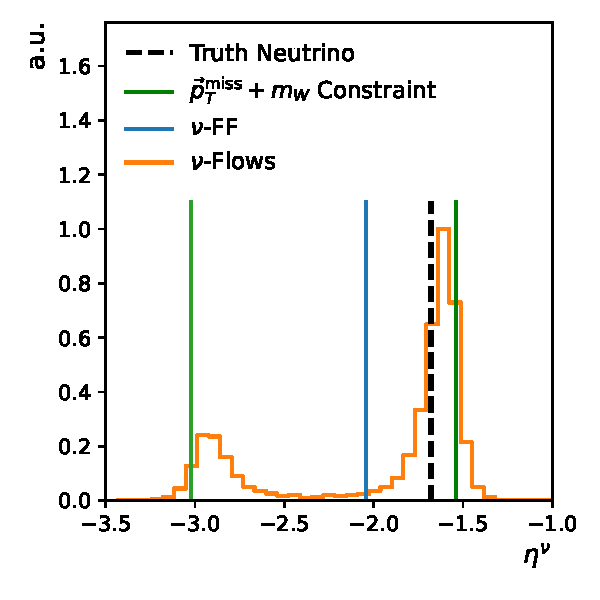
\includegraphics[width=\textwidth]{Figures/neutrino_unfolding/eta_5.pdf}
        \caption{} \label{fig:inf_good}
    \end{subfigure}
        \begin{subfigure}{0.32\textwidth}
        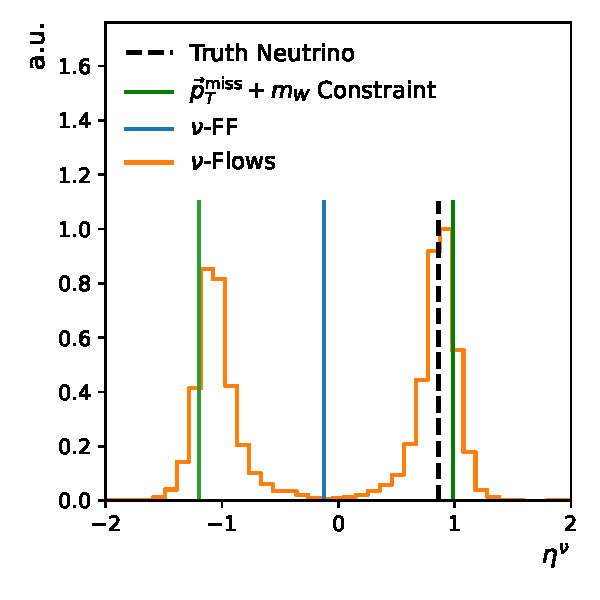
\includegraphics[width=\textwidth]{Figures/neutrino_unfolding/eta_9.pdf}
    \caption{} \label{fig:inf_ambig}
    \end{subfigure}
    \begin{subfigure}{0.32\textwidth}
        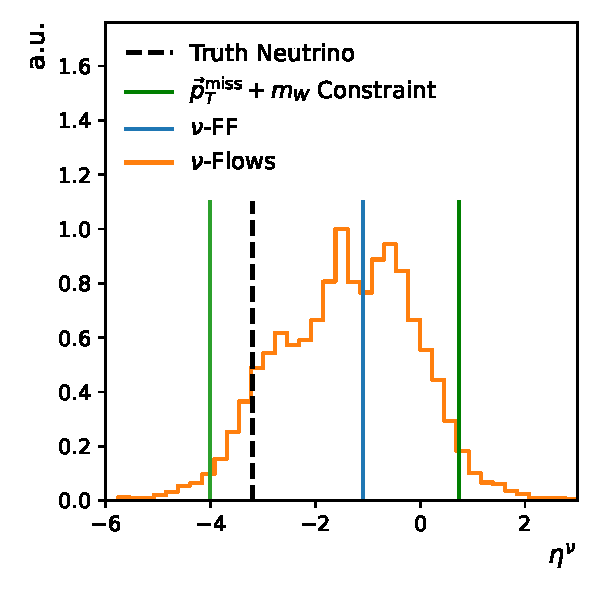
\includegraphics[width=\textwidth]{Figures/neutrino_unfolding/eta_12.pdf}
        \caption{} \label{fig:inf_bad}
    \end{subfigure}
    \caption{The $\eta$ of three different neutrinos selected from the evaluation dataset. The true values are shown in black. The two solutions from the $m_W$ constraint method are shown in green. The single point estimate using \nuff{} is shown in blue. The probability density learned by \nuflow{} is shown in orange.}
    \label{fig:inference}
\end{figure}

\begin{figure}[ht]
    \centering
    \begin{subfigure}{0.40\textwidth}
        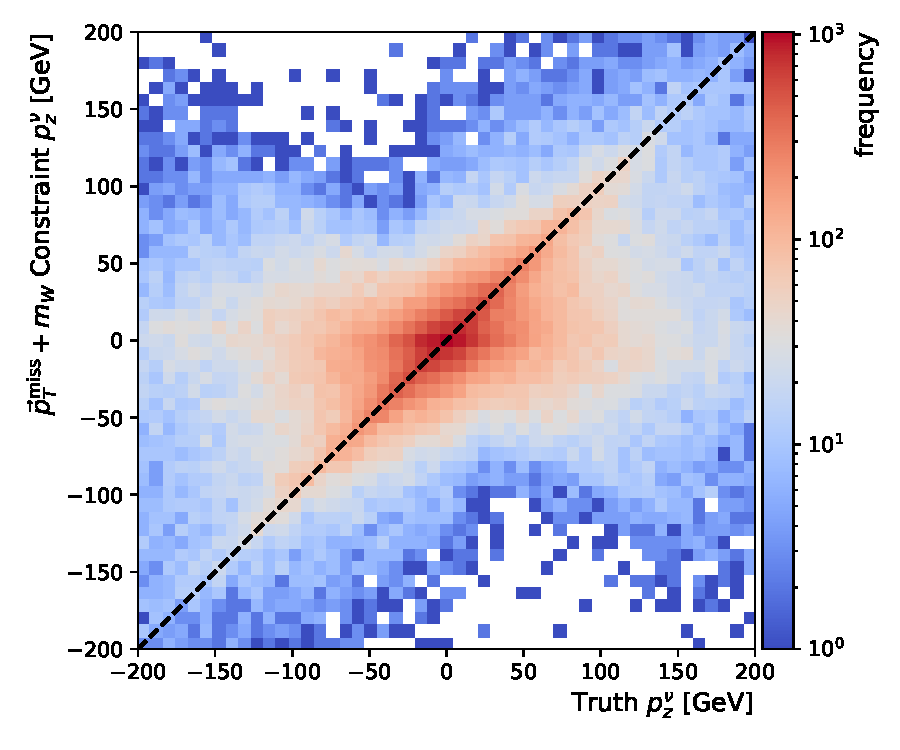
\includegraphics[width=\textwidth]{Figures/neutrino_unfolding/p_z_quad.pdf}
        \caption{} \label{fig:px_dist}
    \end{subfigure}
    \begin{subfigure}{0.40\textwidth}
        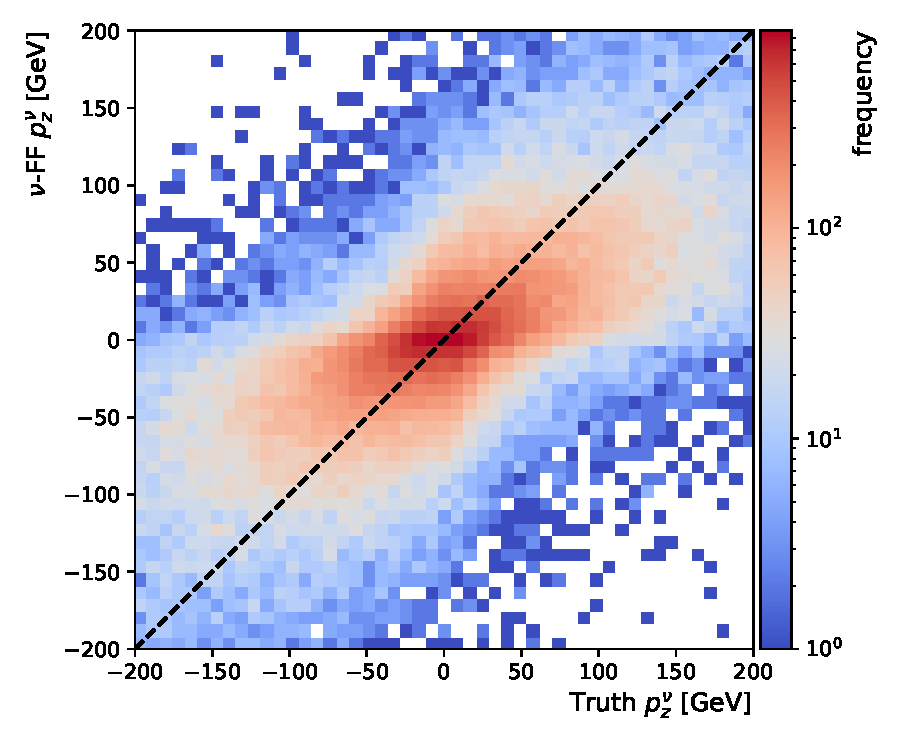
\includegraphics[width=\textwidth]{Figures/neutrino_unfolding/p_z_ff.pdf}
        \caption{} \label{fig:py_dist}
    \end{subfigure}\\
    \begin{subfigure}{0.40\textwidth}
        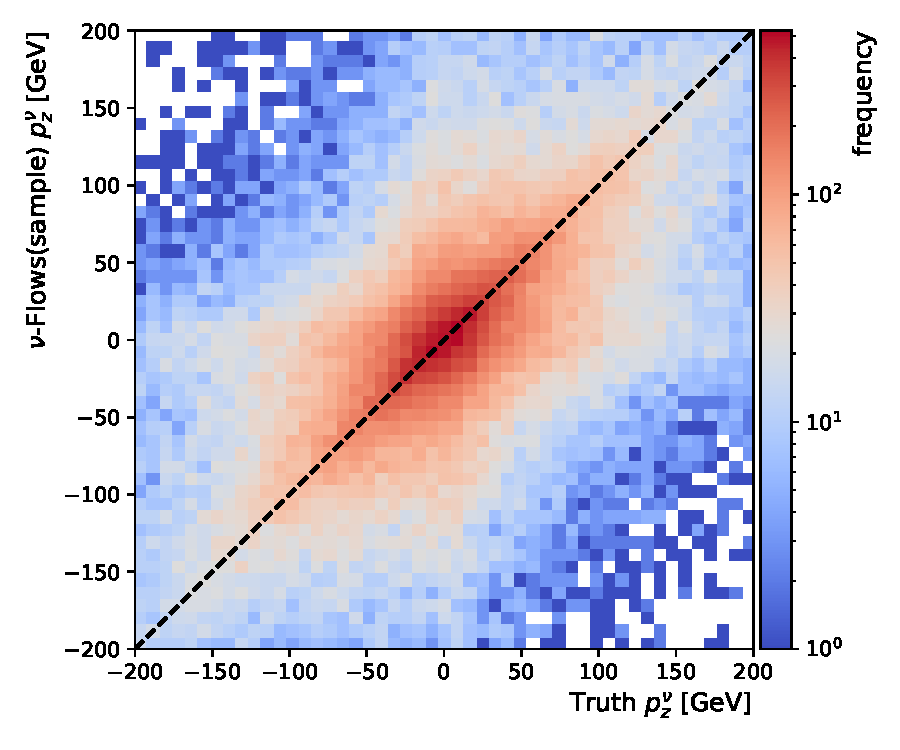
\includegraphics[width=\textwidth]{Figures/neutrino_unfolding/p_z_sample.pdf}
        \caption{} \label{fig:pz_dist}
    \end{subfigure}
    \begin{subfigure}{0.40\textwidth}
        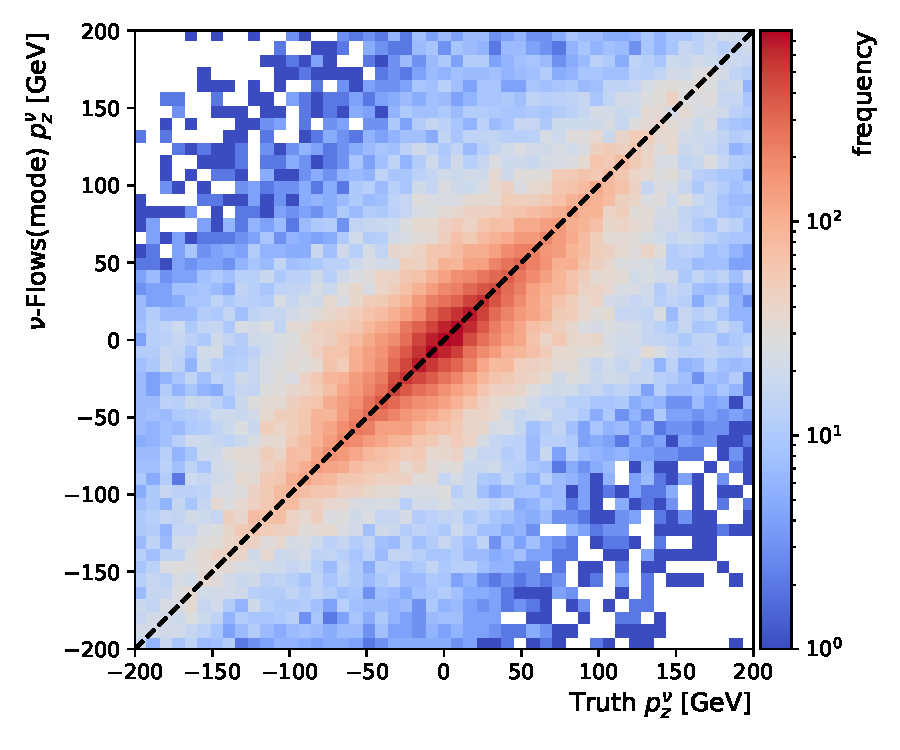
\includegraphics[width=\textwidth]{Figures/neutrino_unfolding/p_z_mode.pdf}
        \caption{} \label{fig:E_dist}
    \end{subfigure}
    \caption{Two-dimensional histograms showing the reconstructed versus true $p_z^\nu$ using the $m_W$ constraint \subref{fig:px_dist}, \nuff{} \subref{fig:py_dist}, \nusample{} \subref{fig:pz_dist}, and \numode{} \subref{fig:E_dist} methods.}
    \label{fig:dists}
\end{figure}

\Cref{fig:lv_mass} shows the reconstructed invariant mass of the leptonic $W$, calculated using the reconstructed lepton and each neutrino estimate.
\nusample{} nearly matches the true neutrino distribution, while \numode{} is centred around the mean.
\nuff{} shows a notable offset of the mean by around $6~\GeV$.
The $m_W$ constraint yields $m_{\ell\nu} = 80.38~\GeV$ for nearly all events, with a positive tail due to no real solutions for the quadratic equation.
The reconstructed invariant mass of the leptonic top quark is shown in \Cref{fig:blv_mass} using the correct $b$-jet from the leptonically decaying top quark to highlight the neutrino reconstruction effect.
Each method shows an increase invariance and a negative bias in the reconstructed mass.
The distribution closest to truth is \nusample.

\begin{figure}[htp]
    \centering
    \begin{subfigure}{0.48\textwidth}
        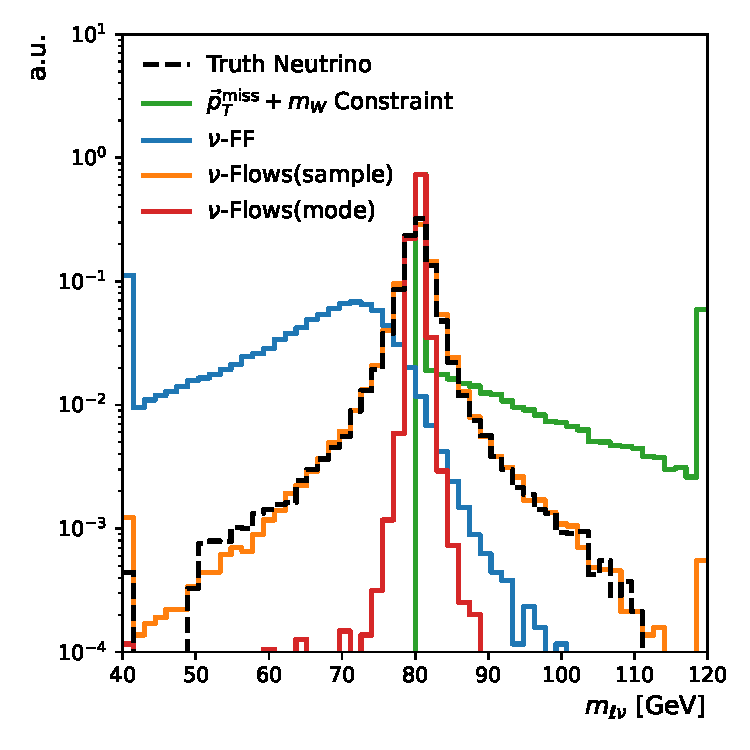
\includegraphics[width=\textwidth]{Figures/neutrino_unfolding/lnu_mass.pdf}
        \caption{} \label{fig:lv_mass}
    \end{subfigure}
        \begin{subfigure}{0.48\textwidth}
        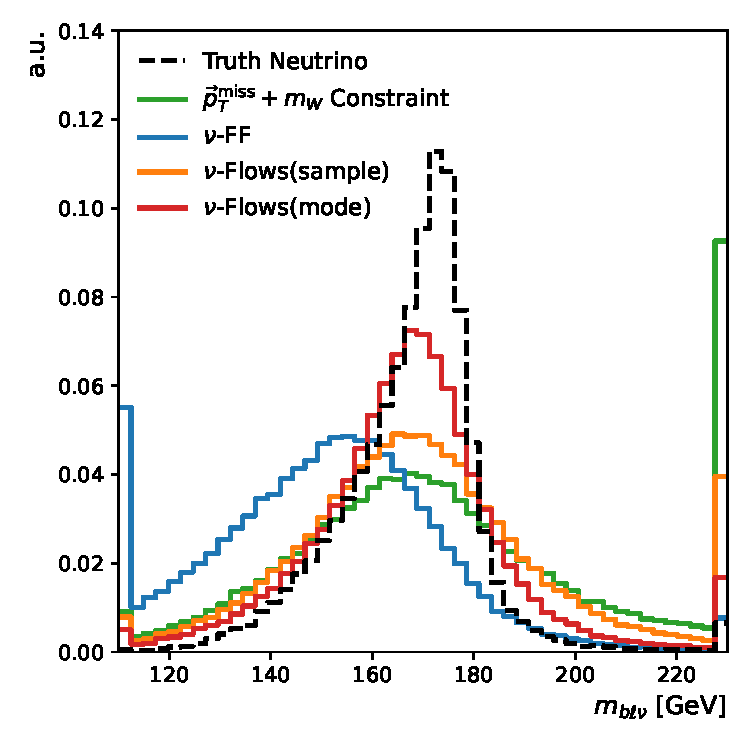
\includegraphics[width=\textwidth]{Figures/neutrino_unfolding/blnu_mass.pdf}
    \caption{} \label{fig:blv_mass}
    \end{subfigure}
    \caption{Distributions of the invariant mass of the $\ell\nu$ \subref{fig:lv_mass} and $b\ell\nu$ \subref{fig:blv_mass} systems using different neutrino reconstruction methods. All methods use reconstructed variables for the lepton and jet kinematics.}
    \label{fig:real_assoc_masses}
\end{figure}

\subsubsection{\texorpdfstring{$\chi^2$}{Chi Squared} Jet Association}

We examine the effect of \nuflow on the combinatoric assignment of jets to final-state partons.
This task is crucial for top quark physics analyses such as measurements of the top quark mass~\cite{ATLAS:2015pfy,CMS:2018quc,ATLAS:2018fwq,ATLAS:2019guf}, differential cross-sections~\cite{CMS:2016oae,CMS:2018htd,ATLAS:2019hxz,CMS:2021vhb}, spin correlation~\cite{CMS:2015cal} and charge asymmetry~\cite{ATLAS:2022waa}.

Semi-leptonic $\ttbar$ events feature four final state partons: $b_{lep}$, $b_{had}$, and the hadronically decaying $W$ boson products, $q_1$ and $q_2$.
The objects may be reconstructed as jets, but so too are signals from initial-state radiation, final-state radiation, and pileup.
Jet assignment often utilizes a $\chi^2$ fit~\cite{Chi2ATLAS}, which is dependent on the neutrino kinematics, underscoring the value of precise neutrino estimation.
This fitting procedure is just one of many jet combinatoric solving methods.
Other methods include KLFitter \cite{KLFitter} or any of the new deep learning approached~\cite{SAJA, SPANet, Spatter, TopoGraphs}.
All of these techniques could also be complemented by \nuflow{}.

In the $\chi^2$ fit method, every possible jet permutation is tested, and the one with the lowest $\chi^2$ value defined by
\begin{equation}
    \chi^2=\frac{(m_W-m_{\ell\nu})^2}{\sigma_{\ell\nu}} +\frac{(m_W-m_{qq})^2}{\sigma_{qq}} +\frac{(m_t-m_{b\ell\nu})^2}{\sigma_{b\ell\nu}} +\frac{(m_t-m_{bqq})^2}{\sigma_{bqq}}
    \label{eq:chi_square}
\end{equation}
is kept.
In this work, the $\sigma$ values are taken from the root-mean-square error of the relevant mass distributions, using the true jet-assignments, and are derived for each neutrino reconstruction method separately.
We perform the $\chi^2$ fit using permutations of up to 9 leading $p_{\mathrm{T}}$ ordered jets and record the parton association accuracy for each neutrino reconstruction method.

The $b_{lep}$ matching efficiency has the highest dependence on the neutrino in the $\chi^2$ fit and the association accuracy of the $b_{lep}$ is shown in Table~\ref{tab:blep_4sig}.
Using estimates from either \nusample{} or \numode{} results in an improved matching efficiency compared to the standard kinematic approach.
The $\chi^2$ fit performed with estimates from \numode{} instead of the $m_W$ constraint led to an increase in accuracy by a factor of $1.03$ for events with four jets and $1.41$ for events with nine jets.
For events with a low number of jets, few permutations exist, which means that the neutrino term is less likely to have an impact in Equation~\ref{eq:chi_square}.
Therefore, the observed relationship between the performance gained using \nuflow{} and the number of jets in the event is expected.
% By improving the jet to parton matching efficiency the measurements of \ttbar event properties will be of direct benefit, and as a result \nuflow{} can be expected to bring improvements to a range of measurements, however future studies will be needed to confirm these expectations.
